%**************************************%
%*    Generated from PreTeXt source   *%
%*    on 2019-06-25T13:07:24-06:00    *%
%*                                    *%
%*      https://pretextbook.org       *%
%*                                    *%
%**************************************%
\documentclass[twoside,11pt,]{book}
%% Custom Preamble Entries, early (use latex.preamble.early)
%% Default LaTeX packages
%%   1.  always employed (or nearly so) for some purpose, or
%%   2.  a stylewriter may assume their presence
\usepackage{geometry}
%% Some aspects of the preamble are conditional,
%% the LaTeX engine is one such determinant
\usepackage{ifthen}
%% etoolbox has a variety of modern conveniences
\usepackage{etoolbox}
\usepackage{ifxetex,ifluatex}
%% Raster graphics inclusion
\usepackage{graphicx}
%% Color support, xcolor package
%% Always loaded, for: add/delete text, author tools
%% Here, since tcolorbox loads tikz, and tikz loads xcolor
\PassOptionsToPackage{usenames,dvipsnames,svgnames,table}{xcolor}
\usepackage{xcolor}
%% Colored boxes, and much more, though mostly styling
%% skins library provides "enhanced" skin, employing tikzpicture
%% boxes may be configured as "breakable" or "unbreakable"
%% "raster" controls grids of boxes, aka side-by-side
\usepackage{tcolorbox}
\tcbuselibrary{skins}
\tcbuselibrary{breakable}
\tcbuselibrary{raster}
%% We load some "stock" tcolorbox styles that we use a lot
%% Placement here is provisional, there will be some color work also
%% First, black on white, no border, transparent, but no assumption about titles
\tcbset{ bwminimalstyle/.style={size=minimal, boxrule=-0.3pt, frame empty,
colback=white, colbacktitle=white, coltitle=black, opacityfill=0.0} }
%% Second, bold title, run-in to text/paragraph/heading
%% Space afterwards will be controlled by environment,
%% dependent of constructions of the tcb title
\tcbset{ runintitlestyle/.style={fonttitle=\normalfont\bfseries, attach title to upper} }
%% Spacing prior to each exercise, anywhere
\tcbset{ exercisespacingstyle/.style={before skip={1.5ex plus 0.5ex}} }
%% Spacing prior to each block
\tcbset{ blockspacingstyle/.style={before skip={2.0ex plus 0.5ex}} }
%% xparse allows the construction of more robust commands,
%% this is a necessity for isolating styling and behavior
%% The tcolorbox library of the same name loads the base library
\tcbuselibrary{xparse}
%% Hyperref should be here, but likes to be loaded late
%%
%% Inline math delimiters, \(, \), need to be robust
%% 2016-01-31:  latexrelease.sty  supersedes  fixltx2e.sty
%% If  latexrelease.sty  exists, bugfix is in kernel
%% If not, bugfix is in  fixltx2e.sty
%% See:  https://tug.org/TUGboat/tb36-3/tb114ltnews22.pdf
%% and read "Fewer fragile commands" in distribution's  latexchanges.pdf
\IfFileExists{latexrelease.sty}{}{\usepackage{fixltx2e}}
%% Text height identically 9 inches, text width varies on point size
%% See Bringhurst 2.1.1 on measure for recommendations
%% 75 characters per line (count spaces, punctuation) is target
%% which is the upper limit of Bringhurst's recommendations
\geometry{letterpaper,total={374pt,9.0in}}
%% Custom Page Layout Adjustments (use latex.geometry)
\geometry{papersize={7in,10in}, width=4.85in, inner=1in, height=8.5in, top=0.75in, twoside, ignoreheadfoot}
%% This LaTeX file may be compiled with pdflatex, xelatex, or lualatex executables
%% LuaTeX is not explicitly supported, but we do accept additions from knowledgeable users
%% The conditional below provides  pdflatex  specific configuration last
%% The following provides engine-specific capabilities
%% Generally, xelatex is necessary non-Western fonts
\ifthenelse{\boolean{xetex} \or \boolean{luatex}}{%
%% begin: xelatex and lualatex-specific configuration
\ifxetex\usepackage{xltxtra}\fi
%% realscripts is the only part of xltxtra relevant to lualatex 
\ifluatex\usepackage{realscripts}\fi
%% fontspec package provides extensive control of system fonts,
%% meaning *.otf (OpenType), and apparently *.ttf (TrueType)
%% that live *outside* your TeX/MF tree, and are controlled by your *system*
%% fontspec will make Latin Modern (lmodern) the default font
\usepackage{fontspec}
%% 
%% Extensive support for other languages
\usepackage{polyglossia}
%% Set main/default language based on pretext/@xml:lang value
%% document language code is "en-US", US English
%% usmax variant has extra hypenation
\setmainlanguage[variant=usmax]{english}
%% Enable secondary languages based on discovery of @xml:lang values
%% Enable fonts/scripts based on discovery of @xml:lang values
%% Western languages should be ably covered by Latin Modern Roman
%% end: xelatex and lualatex-specific configuration
}{%
%% begin: pdflatex-specific configuration
\usepackage[utf8]{inputenc}
%% PreTeXt will create a UTF-8 encoded file
%% begin: font setup and configuration for use with pdflatex
\usepackage{lmodern}
\usepackage[T1]{fontenc}
%% end: font setup and configuration for use with pdflatex
%% end: pdflatex-specific configuration
}
%% Monospace font: Inconsolata (zi4)
%% Sponsored by TUG: http://levien.com/type/myfonts/inconsolata.html
%% Loaded for documents with intentional objects requiring monospace
%% See package documentation for excellent instructions
%% One caveat, seem to need full file name to locate OTF files
%% Loads the "upquote" package as needed, so we don't have to
%% Upright quotes might come from the  textcomp  package, which we also use
%% We employ the shapely \ell to match Google Font version
%% pdflatex: "varqu" option produces best upright quotes
%% xelatex,lualatex: add StylisticSet 1 for shapely \ell
%% xelatex,lualatex: add StylisticSet 2 for plain zero
%% xelatex,lualatex: we add StylisticSet 3 for upright quotes
%% 
\ifthenelse{\boolean{xetex} \or \boolean{luatex}}{%
%% begin: xelatex and lualatex-specific monospace font
\usepackage{zi4}
\setmonofont[BoldFont=Inconsolatazi4-Bold.otf,StylisticSet={1,3}]{Inconsolatazi4-Regular.otf}
%% end: xelatex and lualatex-specific monospace font
}{%
%% begin: pdflatex-specific monospace font
%% "varqu" option provides textcomp \textquotedbl glyph
%% "varl"  option provides shapely "ell"
\usepackage[varqu,varl]{zi4}
%% end: pdflatex-specific monospace font
}
%% Symbols, align environment, bracket-matrix
\usepackage{amsmath}
\usepackage{amssymb}
%% allow page breaks within display mathematics anywhere
%% level 4 is maximally permissive
%% this is exactly the opposite of AMSmath package philosophy
%% there are per-display, and per-equation options to control this
%% split, aligned, gathered, and alignedat are not affected
\allowdisplaybreaks[4]
%% allow more columns to a matrix
%% can make this even bigger by overriding with  latex.preamble.late  processing option
\setcounter{MaxMatrixCols}{30}
%%
%%
%% Division Titles, and Page Headers/Footers
%% titlesec package, loading "titleps" package cooperatively
%% See code comments about the necessity and purpose of "explicit" option
\usepackage[explicit, pagestyles]{titlesec}
\newtitlemark{\chaptertitlename}
%% Set global/default page style for document due
%% to potential re-definitions after documentclass
\pagestyle{headings}
%%
%% Create globally-available macros to be provided for style writers
%% These are redefined for each occurence of each division
\newcommand{\divisionnameptx}{\relax}%
\newcommand{\titleptx}{\relax}%
\newcommand{\subtitleptx}{\relax}%
\newcommand{\shortitleptx}{\relax}%
\newcommand{\authorsptx}{\relax}%
\newcommand{\epigraphptx}{\relax}%
%% Create environments for possible occurences of each division
%% Environment for a PTX "chapter" at the level of a LaTeX "chapter"
\NewDocumentEnvironment{chapterptx}{mmmmmm}
{%
\renewcommand{\divisionnameptx}{Chapter}%
\renewcommand{\titleptx}{#1}%
\renewcommand{\subtitleptx}{#2}%
\renewcommand{\shortitleptx}{#3}%
\renewcommand{\authorsptx}{#4}%
\renewcommand{\epigraphptx}{#5}%
\chapter[#3]{#1}%
\label{#6}%
}{}%
%% Environment for a PTX "worksheet" at the level of a LaTeX "section"
\NewDocumentEnvironment{worksheet-section}{mmmmmm}
{%
\renewcommand{\divisionnameptx}{Worksheet}%
\renewcommand{\titleptx}{#1}%
\renewcommand{\subtitleptx}{#2}%
\renewcommand{\shortitleptx}{#3}%
\renewcommand{\authorsptx}{#4}%
\renewcommand{\epigraphptx}{#5}%
\section[#3]{#1}%
\label{#6}%
}{}%
%% Environment for a PTX "worksheet" at the level of a LaTeX "section"
\NewDocumentEnvironment{worksheet-section-numberless}{mmmmmm}
{%
\renewcommand{\divisionnameptx}{Worksheet}%
\renewcommand{\titleptx}{#1}%
\renewcommand{\subtitleptx}{#2}%
\renewcommand{\shortitleptx}{#3}%
\renewcommand{\authorsptx}{#4}%
\renewcommand{\epigraphptx}{#5}%
\section*{#1}%
\addcontentsline{toc}{section}{#3}
\label{#6}%
}{}%
%%
%% Styles for six traditional LaTeX divisions
\titleformat{\chapter}[display]
{\normalfont\huge\bfseries}{\divisionnameptx\space\thechapter}{20pt}{\Huge#1}
[{\Large\authorsptx}]
\titleformat{name=\chapter,numberless}[display]
{\normalfont\huge\bfseries}{}{0pt}{#1}
[{\Large\authorsptx}]
\titlespacing*{\chapter}{0pt}{50pt}{40pt}
\titleformat{\section}[hang]
{\normalfont\Large\bfseries}{\thesection}{1ex}{#1}
[{\large\authorsptx}]
\titleformat{name=\section,numberless}[block]
{\normalfont\Large\bfseries}{}{0pt}{#1}
[{\large\authorsptx}]
\titlespacing*{\section}{0pt}{3.5ex plus 1ex minus .2ex}{2.3ex plus .2ex}
\titleformat{\subsection}[hang]
{\normalfont\large\bfseries}{\thesubsection}{1ex}{#1}
[{\normalsize\authorsptx}]
\titleformat{name=\subsection,numberless}[block]
{\normalfont\large\bfseries}{}{0pt}{#1}
[{\normalsize\authorsptx}]
\titlespacing*{\subsection}{0pt}{3.25ex plus 1ex minus .2ex}{1.5ex plus .2ex}
\titleformat{\subsubsection}[hang]
{\normalfont\normalsize\bfseries}{\thesubsubsection}{1em}{#1}
[{\small\authorsptx}]
\titleformat{name=\subsubsection,numberless}[block]
{\normalfont\normalsize\bfseries}{}{0pt}{#1}
[{\normalsize\authorsptx}]
\titlespacing*{\subsubsection}{0pt}{3.25ex plus 1ex minus .2ex}{1.5ex plus .2ex}
\titleformat{\paragraph}[hang]
{\normalfont\normalsize\bfseries}{\theparagraph}{1em}{#1}
[{\small\authorsptx}]
\titleformat{name=\paragraph,numberless}[block]
{\normalfont\normalsize\bfseries}{}{0pt}{#1}
[{\normalsize\authorsptx}]
\titlespacing*{\paragraph}{0pt}{3.25ex plus 1ex minus .2ex}{1.5em}
%%
%% Semantic Macros
%% To preserve meaning in a LaTeX file
%%
%% \mono macro for content of "c", "cd", "tag", etc elements
%% Also used automatically in other constructions
%% Simply an alias for \texttt
%% Always defined, even if there is no need, or if a specific tt font is not loaded
\newcommand{\mono}[1]{\texttt{#1}}
%%
%% Following semantic macros are only defined here if their
%% use is required only in this specific document
%%
%% Division Numbering: Chapters, Sections, Subsections, etc
%% Division numbers may be turned off at some level ("depth")
%% A section *always* has depth 1, contrary to us counting from the document root
%% The latex default is 3.  If a larger number is present here, then
%% removing this command may make some cross-references ambiguous
%% The precursor variable $numbering-maxlevel is checked for consistency in the common XSL file
\setcounter{secnumdepth}{1}
%% begin: General AMS environment setup
%% Environments built with amsthm package
\usepackage{amsthm}
%% Numbering for Theorems, Conjectures, Examples, Figures, etc
%% Controlled by  numbering.theorems.level  processing parameter
%% Numbering: all theorem-like numbered consecutively
%% i.e. Corollary 4.3 follows Theorem 4.2
%% Always need some theorem environment to set base numbering scheme
%% even if document has no theorems (but has other environments)
%% Create a never-used style first, always
%% simply to provide a global counter to use, namely "cthm"
\newtheorem{cthm}{BadTheoremStringName}[section]
%% AMS "proof" environment is not used, but we leave previously
%% implemented \qedhere in place, should the LaTeX be recycled
\renewcommand{\qedhere}{\relax}
%% end: General AMS environment setup
%%
%% xparse environments for introductions and conclusions of divisions
%%
%% introduction: in a structured division
\NewDocumentEnvironment{introduction}{m}
{\notblank{#1}{\noindent\textbf{#1}\space}{}}{\par\medskip}
%% Divisional exercises (and worksheet) as LaTeX environments
%% Third argument is option for extra workspace in worksheets
%% Hanging indent occupies a 5ex width slot prior to left margin
%% Experimentally this seems just barely sufficient for a bold "888."
%% Division exercises, not in exercise group
\tcbset{ divisionexercisestyle/.style={bwminimalstyle, runintitlestyle, exercisespacingstyle, left=5ex, breakable, parbox=false } }
\newtcolorbox{divisionexercise}[4]{divisionexercisestyle, before title={\hspace{-5ex}\makebox[5ex][l]{#1.}}, title={\notblank{#2}{#2\space}{}}, phantom={\hypertarget{#4}{}}, after={\notblank{#3}{\newline\rule{\workspacestrutwidth}{#3\textheight}\newline}{}}}
%% Worksheet exercises may have workspaces
\newlength{\workspacestrutwidth}
%% @workspace strut is invisible
\setlength{\workspacestrutwidth}{0pt}
%% Localize LaTeX supplied names (possibly none)
\renewcommand*{\chaptername}{Chapter}
\setcounter{chapter}{-1}
%% "tcolorbox" environment for a single image, occupying entire \linewidth
%% arguments are left-margin, width, right-margin, as multiples of
%% \linewidth, and are guaranteed to be positive and sum to 1.0
\tcbset{ imagestyle/.style={bwminimalstyle} }
\NewTColorBox{image}{mmm}{imagestyle,left skip=#1\linewidth,width=#2\linewidth}
%% For improved tables
\usepackage{array}
%% Some extra height on each row is desirable, especially with horizontal rules
%% Increment determined experimentally
\setlength{\extrarowheight}{0.2ex}
%% Define variable thickness horizontal rules, full and partial
%% Thicknesses are 0.03, 0.05, 0.08 in the  booktabs  package
\newcommand{\hrulethin}  {\noalign{\hrule height 0.04em}}
\newcommand{\hrulemedium}{\noalign{\hrule height 0.07em}}
\newcommand{\hrulethick} {\noalign{\hrule height 0.11em}}
%% We preserve a copy of the \setlength package before other
%% packages (extpfeil) get a chance to load packages that redefine it
\let\oldsetlength\setlength
\newlength{\Oldarrayrulewidth}
\newcommand{\crulethin}[1]%
{\noalign{\global\oldsetlength{\Oldarrayrulewidth}{\arrayrulewidth}}%
\noalign{\global\oldsetlength{\arrayrulewidth}{0.04em}}\cline{#1}%
\noalign{\global\oldsetlength{\arrayrulewidth}{\Oldarrayrulewidth}}}%
\newcommand{\crulemedium}[1]%
{\noalign{\global\oldsetlength{\Oldarrayrulewidth}{\arrayrulewidth}}%
\noalign{\global\oldsetlength{\arrayrulewidth}{0.07em}}\cline{#1}%
\noalign{\global\oldsetlength{\arrayrulewidth}{\Oldarrayrulewidth}}}
\newcommand{\crulethick}[1]%
{\noalign{\global\oldsetlength{\Oldarrayrulewidth}{\arrayrulewidth}}%
\noalign{\global\oldsetlength{\arrayrulewidth}{0.11em}}\cline{#1}%
\noalign{\global\oldsetlength{\arrayrulewidth}{\Oldarrayrulewidth}}}
%% Single letter column specifiers defined via array package
\newcolumntype{A}{!{\vrule width 0.04em}}
\newcolumntype{B}{!{\vrule width 0.07em}}
\newcolumntype{C}{!{\vrule width 0.11em}}
%% Figures, Tables, Listings, Named Lists, Floats
%% The [H]ere option of the float package fixes floats in-place,
%% in deference to web usage, where floats are totally irrelevant
%% You can remove some of this setup, to restore standard LaTeX behavior
%% HOWEVER, numbering of figures/tables AND theorems/examples/remarks, etc
%% may de-synchronize with the numbering in the HTML version
%% You can remove the "placement={H}" option to allow flotation and
%% preserve numbering, BUT the numbering may then appear "out-of-order"
%% Floating environments: http://tex.stackexchange.com/questions/95631/
\usepackage{float}
\usepackage{newfloat}
\usepackage{caption}%% Adjust stock figure environment so that it no longer floats
\SetupFloatingEnvironment{figure}{fileext=lof,placement={H},within=section,name=Figure}
\captionsetup[figure]{labelfont=bf}
%% http://tex.stackexchange.com/questions/16195
\makeatletter
\let\c@figure\c@cthm
\makeatother
%% Adjust stock table environment so that it no longer floats
\SetupFloatingEnvironment{table}{fileext=lot,placement={H},within=section,name=Table}
\captionsetup[table]{labelfont=bf}
%% http://tex.stackexchange.com/questions/16195
\makeatletter
\let\c@table\c@cthm
\makeatother
%% More flexible list management, esp. for references
%% But also for specifying labels (i.e. custom order) on nested lists
\usepackage{enumitem}
%% hyperref driver does not need to be specified, it will be detected
%% Footnote marks in tcolorbox have broken linking under
%% hyperref, so it is necessary to turn off all linking
%% It *must* be given as a package option, not with \hypersetup
\usepackage[hyperfootnotes=false]{hyperref}
%% configure hyperref's  \url  to match listings' inline verbatim
\renewcommand\UrlFont{\small\ttfamily}
%% Hyperlinking active in electronic PDFs, all links solid and blue
\hypersetup{colorlinks=true,linkcolor=blue,citecolor=blue,filecolor=blue,urlcolor=blue}
\hypersetup{pdftitle={Mathematics for Elementary Teachers}}
%% If you manually remove hyperref, leave in this next command
\providecommand\phantomsection{}
%% Graphics Preamble Entries
\usepackage{tikz, pgfplots}
\usetikzlibrary{positioning,matrix,arrows}
\usetikzlibrary{shapes,decorations,shadows,fadings,patterns}
\usetikzlibrary{decorations.markings}
%% If tikz has been loaded, replace ampersand with \amp macro
%% tcolorbox styles for sidebyside layout
\tcbset{ sbsstyle/.style={raster equal height=rows,raster force size=false} }
\tcbset{ sbsheadingstyle/.style={bwminimalstyle, halign=center, fontupper=\bfseries} }
\tcbset{ sbspanelstyle/.style={bwminimalstyle} }
\tcbset{ sbscaptionstyle/.style={bwminimalstyle, halign=center} }
%% Enviroments for side-by-side and components
%% Necessary to use \NewTColorBox for boxes of the panels
%% "newfloat" environment to squash page-breaks within a single sidebyside
%% \leavevmode necessary when a side-by-side comes first, right after a heading
%% "xparse" environment for entire sidebyside
\NewDocumentEnvironment{sidebyside}{mmmm}
  {\begin{tcbraster}
    [sbsstyle,raster columns=#1,
    raster left skip=#2\linewidth,raster right skip=#3\linewidth,raster column skip=#4\linewidth]}
  {\end{tcbraster}}
%% "tcolorbox" environments for three components of a panel
\NewTColorBox{sbsheading}{m}{sbsheadingstyle,width=#1\linewidth}
\NewTColorBox{sbspanel}{mO{top}}{sbspanelstyle,width=#1\linewidth,valign=#2}
\NewTColorBox{sbscaption}{m}{sbscaptionstyle,width=#1\linewidth}
%% extpfeil package for certain extensible arrows,
%% as also provided by MathJax extension of the same name
%% NB: this package loads mtools, which loads calc, which redefines
%%     \setlength, so it can be removed if it seems to be in the 
%%     way and your math does not use:
%%     
%%     \xtwoheadrightarrow, \xtwoheadleftarrow, \xmapsto, \xlongequal, \xtofrom
%%     
%%     we have had to be extra careful with variable thickness
%%     lines in tables, and so also load this package late
\usepackage{extpfeil}
%% Custom Preamble Entries, late (use latex.preamble.late)
%% Begin: Author-provided packages
%% (From  docinfo/latex-preamble/package  elements)
%% End: Author-provided packages
%% Begin: Author-provided macros
%% (From  docinfo/macros  element)
%% Plus three from MBX for XML characters
\newcommand{\N}{\mathbb N}
\newcommand{\Z}{\mathbb Z}
\newcommand{\Q}{\mathbb Q}
\newcommand{\R}{\mathbb R}
\newcommand{\C}{\mathbb C}
\newcommand{\inv}{^{-1}}
\newcommand{\st}{:}
\renewcommand{\iff}{\leftrightarrow}
\newcommand{\Iff}{\Leftrightarrow}
\newcommand{\imp}{\rightarrow}
\newcommand{\Imp}{\Rightarrow}
\newcommand{\isom}{\cong}

\renewcommand{\bar}{\overline}
\newcommand{\card}[1]{\left| #1 \right|}
\newcommand{\lt}{<}
\newcommand{\gt}{>}
\newcommand{\amp}{&}
%% End: Author-provided macros
\begin{document}
\frontmatter
%% begin: half-title
\thispagestyle{empty}
{\centering
\vspace*{0.28\textheight}
{\Huge Mathematics for Elementary Teachers}\\[2\baselineskip]
{\LARGE A Workbook}\\
}
\clearpage
%% end:   half-title
%% begin: adcard
\thispagestyle{empty}
\null%
\clearpage
%% end:   adcard
%% begin: title page
%% Inspired by Peter Wilson's "titleDB" in "titlepages" CTAN package
\thispagestyle{empty}
{\centering
\vspace*{0.14\textheight}
%% Target for xref to top-level element is ToC
\addtocontents{toc}{\protect\hypertarget{book-502359955440}{}}
{\Huge Mathematics for Elementary Teachers}\\[\baselineskip]
{\LARGE A Workbook}\\[3\baselineskip]
{\Large \textbraceleft{}author\textbraceright{}}\\[0.5\baselineskip]
{\Large \textbraceleft{}institution\textbraceright{}}\\[3\baselineskip]
{\Large June 25, 2019}\\}
\clearpage
%% end:   title page
%% begin: copyright-page
\thispagestyle{empty}
\hypertarget{colophon-502359931120}{}\vspace*{\stretch{2}}
\noindent{\bfseries Website}: \href{[website]}{\mono{[website]}}\par\medskip
\noindent\textcopyright{}[copyright-year]\quad{}[copyright-holder]\\[0.5\baselineskip]
 This work is licensed under the Creative Commons Attribution-ShareAlike 4.0 International License. To view a copy of this license, visit \href{http://creativecommons.org/licenses/by-sa/4.0/}{http:\slash{}\slash{}creativecommons.org\slash{}licenses\slash{}by-sa\slash{}4.0\slash{}}\par\medskip
\vspace*{\stretch{1}}
\null\clearpage
%% end:   copyright-page
%% begin: table of contents
%% Adjust Table of Contents
\setcounter{tocdepth}{2}
\renewcommand*\contentsname{Contents}
\tableofcontents
%% end:   table of contents
\mainmatter
%
%
\typeout{************************************************}
\typeout{Chapter 0 Worksheets}
\typeout{************************************************}
%
\begin{chapterptx}{Worksheets}{}{Worksheets}{}{}{chapter-502359953616}
%
%
\typeout{************************************************}
\typeout{Worksheet 0 Pizza Splitting Problem}
\typeout{************************************************}
%
\newgeometry{left=1.25cm, right=1.25cm, top=1.25cm, bottom=1.25cm}
\begin{worksheet-section-numberless}{Pizza Splitting Problem}{}{Pizza Splitting Problem}{}{}{worksheet-502359944672}
\begin{introduction}{}%
\hypertarget{p-502359934960}{}%
At a birthday party everyone is about to sit down for pizza.  All the pizzas in this problem are the same size, and the same toppings are distributed evenly on all pizzas.%
\end{introduction}%
\hypertarget{p-502359915392}{}%
(Quick Warm UP Problem) At one table there are 4 pizzas and 8 chairs.  At the other table there are 4 pizzas and 10 chairs.  Carlos knows that everyone at the party is pretty hungry, and assumes that the pizzas at each table will be split evenly, so he wants to sit at the table at which he will end up with the most pizza.  Which table should he choose?  Assume that the pizzas are uncut until all chairs at the table are occupied.%
\begin{divisionexercise}{1}{}{0.1}{exercise-502359914560}%
\hypertarget{p-502359913920}{}%
What if, at one table there are 3 pizzas and 8 chairs, and at the other table there are 4 pizzas and 10 chairs.  Carlos, again, knows that everyone at the party is pretty hungry, and assumes that the pizzas at each table will be split evenly.  He still wants to sit at the table at which he will end up with the most pizza.  Which table should he choose in this situation? Assume that the pizzas are uncut until all chairs at the table are occupied.%
\end{divisionexercise}%
\begin{divisionexercise}{2}{}{0.1}{exercise-502359912800}%
\hypertarget{p-502359912160}{}%
Now, assume that each pizza is already cut into 12 equal pieces. At one table there are 3 pizzas and 8 chairs.  At the other table there are 4 pizzas and 10 chairs.  Which table should he choose?%
\end{divisionexercise}%
\begin{divisionexercise}{3}{}{0.1}{exercise-502359911296}%
\hypertarget{p-502359910656}{}%
Suppose now that, instead of dividing up the pizza separately at each table, the hosts decide to give all 18 people equal amounts from the 7 pizzas.  Carlos realizes that this means that the amount everyone ends up with is in between the amounts they would have ended up with if each pizza had only been shared among those at the same table.  How can we state this observation in terms of fractions?  How can we state this observation in terms of straight-line graphs?  Is there a general relationship about fractions that this is illustrating?  Is there a general graphical relationship that this is illustrating?%
\end{divisionexercise}%
\clearpage
\begin{divisionexercise}{4}{}{0.1}{exercise-502359909056}%
\hypertarget{p-502359908272}{}%
Maria solved problem 2 on handout 1 by using graph paper and drawing two straight lines.  She is wondering what the lines represent, what their equations are and what other problems could be solved with them, now that the lines are drawn.  She is also wondering what the slope of each line represents.  What can we tell Maria on these questions?%
\begin{sidebyside}{1}{0.05}{0.05}{0}%
\begin{sbspanel}{0.9}%
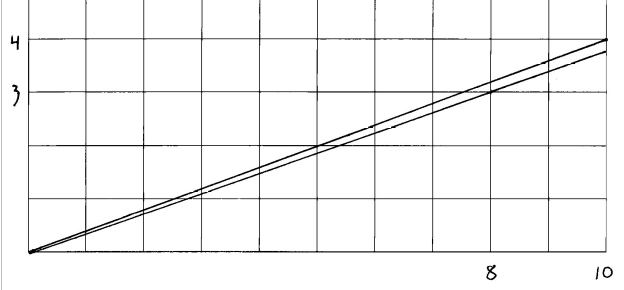
\includegraphics[width=1\linewidth]{images/pizza-splitting-problem.png}
\end{sbspanel}%
\end{sidebyside}%
\end{divisionexercise}%
\begin{divisionexercise}{5}{}{}{exercise-502359906016}%
\hypertarget{p-502359905472}{}%
(Problem 2 on Handout 1) At one table there are 3 pizzas and 8 chairs, and at the other table there are 4 pizzas and 10 chairs.  Carlos, again, knows that everyone at the party is pretty hungry, and assumes that the pizzas at each table will be split evenly, he still wants to sit at the table at which he will end up with the most pizza.  Which table should he choose in this situation? Assume that the pizzas are uncut until all chairs at the table are occupied.%
\end{divisionexercise}%
\begin{divisionexercise}{6}{}{}{exercise-502359904288}%
\hypertarget{p-502359903744}{}%
Create and interpret a double number line way to solve this problem.%
\end{divisionexercise}%
\begin{divisionexercise}{7}{}{}{exercise-502359902960}%
\hypertarget{p-502359902416}{}%
Create and interpret a People vs Pizza graph to solve this problem, and relate it to the previous double number line.%
\end{divisionexercise}%
\end{worksheet-section-numberless}
\restoregeometry
%
%
\typeout{************************************************}
\typeout{Worksheet 0 A Trip to Quintopia!}
\typeout{************************************************}
%
\newgeometry{left=1.25cm, right=1.25cm, top=1.25cm, bottom=1.25cm}
\begin{worksheet-section-numberless}{A Trip to Quintopia!}{}{A Trip to Quintopia!}{}{}{worksheet-502359943168}
\begin{introduction}{}%
\hypertarget{p-502359932992}{}%
While on an Intergalactic Numismatics Tour, you encounter a meteor shower and are forced to make an unscheduled stop on the planet Quintopia.  The monetary system used in Quintopia consists of three coins:  a yellow coin (worth \textdollar{}1US), a red coin (worth five yellow coins), and a blue coin (worth five red coins).%
\par
\hypertarget{p-502359891328}{}%
Quintopia turns out to be a rather dull place to visit.  To help pass the time at the shuttle docking area, you and a fellow passenger play a game with the Quintopia currency.%
\end{introduction}%
\begin{divisionexercise}{1}{}{0.1}{exercise-502359890624}%
\hypertarget{p-502359889984}{}%
Coin Trading Game%
\par
\hypertarget{p-502359889600}{}%
Materials:  Quintopia coins (yellow, red and blue), one die (number cube)%
\par
\hypertarget{p-502359889216}{}%
Players:  2 or more%
\par
\hypertarget{p-502359888832}{}%
Rules:  The youngest player starts, and players alternate turns afterwards.%
\par
\hypertarget{p-502359888352}{}%
On each turn, a player rolls the die and places that many yellow coins on his or her game sheet (see below).%
\par
\hypertarget{p-502359887840}{}%
Whenever possible, a player MUST trade in five yellow coins for a red coin, or trade in five red coins for a blue coin, and place them in their respective columns.  As a result, no more than four coins of any one color should be a player’s game sheet.%
\par
\hypertarget{p-502359887184}{}%
The first player to get two blue coins is the winner.%
\begin{table}
\centering
\begin{tabular}{lll}
BLUE&RED&YELLOW\tabularnewline[0pt]
&&
\end{tabular}
\end{table}
\end{divisionexercise}%
\clearpage
\begin{divisionexercise}{2}{}{0.1}{exercise-502359879920}%
\hypertarget{p-502359879136}{}%
Coin Trading Game Revisited%
\par
\hypertarget{p-502359878704}{}%
A third passenger has been watching you play.  She suggests it is more challenging to start the game with TWO BLUE coins and to remove the number of yellow coins equal to the number rolled on each turn.  The first player to remove all of the coins from his or her playing board is the winner.  (Note: On the last turn, the number rolled may exceed the number of yellow chips remaining.)  Before you play this new version of the coin trading game, think about how you can remove yellow coins when you have none on your board (you only have two blue ones).  Note: Do not trade in coins until you absolutely need to.  For example, you should not immediately trade in your two blue coins all for red or yellow coins.%
\begin{table}
\centering
\begin{tabular}{lll}
BLUE&RED&YELLOW\tabularnewline[0pt]
&&
\end{tabular}
\end{table}
\hypertarget{p-502359871632}{}%
What do you notice?%
\par
\hypertarget{p-502359871200}{}%
What do you wonder?%
\par
\hypertarget{p-502359870768}{}%
What ideas do you have?%
\end{divisionexercise}%
\end{worksheet-section-numberless}
\restoregeometry
%
%
\typeout{************************************************}
\typeout{Worksheet 0 Shopping in Quintopia}
\typeout{************************************************}
%
\newgeometry{left=1.25cm, right=1.25cm, top=1.25cm, bottom=1.25cm}
\begin{worksheet-section-numberless}{Shopping in Quintopia}{}{Shopping in Quintopia}{}{}{worksheet-502359920848}
\begin{introduction}{}%
\hypertarget{p-502359924928}{}%
You got bored on the ship deck and decided to visit Quintopia to do some shopping. You know you can only use Quintopian currency while shopping, so you exchange some of your US dollars before your shopping and you have \(312_{5}\) (in Quintopian currency), which means 3 blue, 1 red, and 2 yellow coins. While you’re shopping, recall that whenever possible, you must trade in five yellow coins for a red coin, or trade in five red coins for a blue coin, and so on.%
\end{introduction}%
\begin{divisionexercise}{1}{}{0.1}{exercise-502359922128}%
\hypertarget{p-502359921488}{}%
Before you left the ship, you won a gift card worth \(24_{5}\) (in Quintopian currency). How much total money do you have now for shopping? Show your process at least in two different ways.%
\end{divisionexercise}%
\begin{divisionexercise}{2}{}{0.1}{exercise-502359919584}%
\hypertarget{p-502359918944}{}%
You spent \(43_{5}\) at the Appletopia store. How much Quintopian money do you have left?  Explain your process.%
\end{divisionexercise}%
\begin{divisionexercise}{3}{}{0.1}{exercise-502359917760}%
\hypertarget{p-502359916976}{}%
You saw a pair of shoes you like and it only costs \(32_{5}\). Since it is very cheap, you want to buy three pairs. How much will it cost to buy three pairs of shoes (in Quintopia currency)? Solve this question in two different ways.%
\end{divisionexercise}%
\clearpage
\begin{divisionexercise}{4}{}{0.1}{exercise-502359869456}%
\hypertarget{p-502359868672}{}%
After buying all three pairs of shoes, how much money do you have left?%
\end{divisionexercise}%
\begin{divisionexercise}{5}{}{0.1}{exercise-502359867904}%
\hypertarget{p-502359867120}{}%
After all your shopping you had some dinner which cost \(102_{5}\) . Do you have enough Quintopian money to pay? If not, how much Quintopian money do you need?  If you have an extra \textdollar{}6 US currency, will that be enough to pay the rest?%
\end{divisionexercise}%
\begin{divisionexercise}{6}{}{0.1}{exercise-502359865792}%
\hypertarget{p-502359865008}{}%
Discuss Base 5 and Base 10; and meaning of addition, subtraction and multiplication operations. Discuss expanded form.%
\end{divisionexercise}%
\end{worksheet-section-numberless}
\restoregeometry
%
%
\typeout{************************************************}
\typeout{Worksheet 0 Connections to Base Blocks}
\typeout{************************************************}
%
\newgeometry{left=1.25cm, right=1.25cm, top=1.25cm, bottom=1.25cm}
\begin{worksheet-section-numberless}{Connections to Base Blocks}{}{Connections to Base Blocks}{}{}{worksheet-502359898256}
\begin{divisionexercise}{1}{}{0.1}{exercise-502359923776}%
\hypertarget{p-502359923136}{}%
Using base-5 blocks, discuss how Quintopian currency would be represented. For example, represent \(314_{5}\) and \(43_{5}\). If you have \textdollar{}58 dollars how would you represent it using base-5 blocks?%
\end{divisionexercise}%
\begin{divisionexercise}{2}{}{0.1}{exercise-502359861360}%
\hypertarget{p-502359860624}{}%
If you have \(412_{5}\) in base-5 blocks and you trade in all the blocks for their corresponding number of small cubes, how many small cubes would you have?%
\end{divisionexercise}%
\begin{divisionexercise}{3}{}{0.1}{exercise-502359859360}%
\hypertarget{p-502359858576}{}%
Discuss with your group.%
\leavevmode%
\begin{enumerate}[label=(\alph*)]
\item\hypertarget{li-502359857616}{}How do base-5 blocks compare to base-10?%
\item\hypertarget{li-502359857152}{}What are the place values worth in base-5 vs. base-10?%
\item\hypertarget{li-502359856672}{}What are the minimum and maximum number of blocks of each place value that you can have in base-5?%
\item\hypertarget{li-502359856144}{}What about base-10?%
\item\hypertarget{li-502359855696}{}How does this relate to the digits you can use to represent numbers in base-5 vs. base-10?%
\end{enumerate}
\end{divisionexercise}%
\begin{divisionexercise}{4}{}{0.1}{exercise-502359854752}%
\hypertarget{p-502359853968}{}%
Using base-10 blocks find the sum and the difference of 208 and 93.%
\end{divisionexercise}%
\begin{divisionexercise}{5}{}{0.1}{exercise-502359853184}%
\hypertarget{p-502359852400}{}%
List multiple things that you observe that are similar and different between addition and subtraction in base 5 (Quintopia) compared to base 10.%
\end{divisionexercise}%
\end{worksheet-section-numberless}
\restoregeometry
%
%
\typeout{************************************************}
\typeout{Worksheet 0 Algorithms for Addition and Subtraction}
\typeout{************************************************}
%
\newgeometry{left=1.25cm, right=1.25cm, top=1.25cm, bottom=1.25cm}
\begin{worksheet-section-numberless}{Algorithms for Addition and Subtraction}{}{Algorithms for Addition and Subtraction}{}{}{worksheet-502359896000}
\begin{divisionexercise}{1}{}{0.1}{exercise-502359863584}%
\hypertarget{p-502359862928}{}%
Carry out the steps of the usual addition algorithm in the problems below in base 5.  Carefully EXPLAIN what each of the ``carried'' (regrouped or traded in) numbers mean.  You may want to refer to base 5 blocks in your explanation.%
\par
\hypertarget{p-502359899312}{}%
%
\begin{equation*}
43_{5}+12_{5} \text{ and } 243_{5}+324_{5}
\end{equation*}
%
\end{divisionexercise}%
\clearpage
\begin{divisionexercise}{2}{}{0.1}{exercise-502359937408}%
\hypertarget{p-502359936624}{}%
Carry out the steps of the usual subtraction algorithm in the problem below using base 5.  Carefully EXPLAIN what each of the ``borrowed'' (regrouped or traded in) numbers means.  You may want to refer to base 5 blocks in your explanation.%
\begin{equation*}
321_{5}-124_5 \text{ and } 301_5-213_5 \text{.}
\end{equation*}
%
\end{divisionexercise}%
\end{worksheet-section-numberless}
\restoregeometry
%
%
\typeout{************************************************}
\typeout{Worksheet 0 Different Bases}
\typeout{************************************************}
%
\newgeometry{left=1.25cm, right=1.25cm, top=1.25cm, bottom=1.25cm}
\begin{worksheet-section-numberless}{Different Bases}{}{Different Bases}{}{}{worksheet-502359897808}
\begin{divisionexercise}{1}{}{0.1}{exercise-502359900960}%
\hypertarget{p-502359900320}{}%
In the base-7 number system, the amount: 1 flat, 6 longs, and 5 small cubes is recorded as \(165_{seven}\) or \(165_7\). In general, we record the base as a subscript except for base 10, since that is the assumed standard base.  Note that in base-7, 1 long is worth 7 small cubes, and 1 flat is worth 7 longs (which is 49 small cubes).%
\par
\hypertarget{p-502359832400}{}%
For each number below, determine how many small cubes that number would consist of if we traded in all the base blocks for their corresponding number of small cubes.  In other words, what amount of small cubes is represented by each number in its corresponding base?%
\leavevmode%
\begin{enumerate}[label=(\alph*)]
\item\hypertarget{li-502359831248}{}\(1202_{three}   = \)%
\item\hypertarget{li-502359830720}{}\(53_{seven}       = \)%
\item\hypertarget{li-502359830016}{}\(203_{four}       = \)%
\item\hypertarget{li-502359829312}{}\(10111_{two}       = \)%
\end{enumerate}
\end{divisionexercise}%
\begin{divisionexercise}{2}{}{0.1}{exercise-502359828176}%
\hypertarget{p-502359827392}{}%
What are the place values after the decimal point in base 10? For example, write the expanded form of 1.29 to show the place values. What about the place values in base 5 after the decimal point (e.g., 12.345) ?%
\end{divisionexercise}%
\begin{divisionexercise}{3}{}{0.1}{exercise-502359826480}%
\hypertarget{p-502359825696}{}%
Write the following numbers in expanded form:%
\leavevmode%
\begin{enumerate}[label=(\alph*)]
\item\hypertarget{li-502359824736}{}\(3,189.208 = \)%
\item\hypertarget{li-502359824192}{}\(34.21_5      = \)%
\end{enumerate}
\end{divisionexercise}%
\begin{divisionexercise}{4}{}{0.1}{exercise-502359823072}%
\hypertarget{p-502359822288}{}%
What are the place values in base six?  What digits are needed?%
\end{divisionexercise}%
\begin{divisionexercise}{5}{}{0.1}{exercise-502359821536}%
\hypertarget{p-502359820752}{}%
How do you immediately know there is an error in each statement?  How would we correctly represent these amounts in the given bases?%
\leavevmode%
\begin{enumerate}[label=(\alph*)]
\item\hypertarget{li-502359819696}{}eleven \(= 32_{three}\)%
\item\hypertarget{li-502359819008}{}fifty-seven \(= 108_{seven}\)%
\end{enumerate}
\end{divisionexercise}%
\begin{divisionexercise}{6}{}{0.1}{exercise-502359817744}%
\hypertarget{p-502359816960}{}%
In base 6, a particular number can be made with 10 large cubes, 9 flats, 7 longs, and 5 small cubes.  What is this number in base 6? (Hint: the answer is NOT \(10975_6 \). Try to solve this without converting to base 10)?%
\end{divisionexercise}%
\begin{divisionexercise}{7}{}{0.1}{exercise-502359815648}%
\hypertarget{p-502359814864}{}%
My last digit is a 0 when I am represented in base-5 and a 1 when represented in base-2.  What is my last digit when represented base-10? Explain.%
\end{divisionexercise}%
\end{worksheet-section-numberless}
\restoregeometry
%
%
\typeout{************************************************}
\typeout{Worksheet 0 Extra Practice: Addition and Subtraction in Other Bases}
\typeout{************************************************}
%
\newgeometry{left=1.25cm, right=1.25cm, top=1.25cm, bottom=1.25cm}
\begin{worksheet-section-numberless}{Extra Practice: Addition and Subtraction in Other Bases}{}{Extra Practice: Addition and Subtraction in Other Bases}{}{}{worksheet-502359896384}
\begin{divisionexercise}{1}{}{0.1}{exercise-502359847200}%
\hypertarget{p-502359848112}{}%
Carry out the steps of the usual addition algorithm in the problem below in the designated base.  Carefully EXPLAIN what each of the “carried” (regrouped\slash{}traded in) numbers mean.  You may want to refer to the appropriate base blocks in your explanation.%
\par
\hypertarget{p-502359839984}{}%
\(33_4+12_4\) and \(263_7+324_7\)%
\end{divisionexercise}%
\begin{divisionexercise}{2}{}{0.1}{exercise-502359838832}%
\hypertarget{p-502359838144}{}%
Carry out the steps of the usual subtraction algorithm in the problem below in the designated base.  Carefully EXPLAIN what each of the “borrowed” (regrouped\slash{}traded in) numbers means.  You may want to refer to the appropriate base blocks in your explanation.%
\par
\hypertarget{p-502359837472}{}%
\(341_8 - 154_8 \) and \(301_4 -213_4\)%
\end{divisionexercise}%
\end{worksheet-section-numberless}
\restoregeometry
%
%
\typeout{************************************************}
\typeout{Worksheet 0 Mental Math and Properties of Addition}
\typeout{************************************************}
%
\newgeometry{left=1.25cm, right=1.25cm, top=1.25cm, bottom=1.25cm}
\begin{worksheet-section-numberless}{Mental Math and Properties of Addition}{}{Mental Math and Properties of Addition}{}{}{worksheet-502359845056}
\begin{introduction}{}%
\hypertarget{p-502359846320}{}%
Try to find ways that make the following problems easy to do mentally.%
\end{introduction}%
\begin{divisionexercise}{1}{}{0.08}{exercise-502359845808}%
\hypertarget{p-502359812176}{}%
%
\begin{equation*}
7999+857+1
\end{equation*}
%
\end{divisionexercise}%
\begin{divisionexercise}{2}{}{0.08}{exercise-502359811104}%
\hypertarget{p-502359810320}{}%
%
\begin{equation*}
367+98+2
\end{equation*}
%
\end{divisionexercise}%
\begin{divisionexercise}{3}{}{0.08}{exercise-502359809200}%
\hypertarget{p-502359808416}{}%
%
\begin{equation*}
153+19+7
\end{equation*}
%
\end{divisionexercise}%
\begin{divisionexercise}{4}{}{0.08}{exercise-502359807296}%
\hypertarget{p-502359806512}{}%
%
\begin{equation*}
7.89+6.93+0.07
\end{equation*}
%
\end{divisionexercise}%
\begin{divisionexercise}{5}{}{0.08}{exercise-502359805392}%
\hypertarget{p-502359804608}{}%
%
\begin{equation*}
37-14-7
\end{equation*}
%
\end{divisionexercise}%
\begin{divisionexercise}{6}{}{0.08}{exercise-502359803488}%
\hypertarget{p-502359802704}{}%
%
\begin{equation*}
91-23-3
\end{equation*}
%
\end{divisionexercise}%
\end{worksheet-section-numberless}
\restoregeometry
%
%
\typeout{************************************************}
\typeout{Worksheet 0 Addition and Subtraction on Number Lines and Different Strategies}
\typeout{************************************************}
%
\newgeometry{left=1.25cm, right=1.25cm, top=1.25cm, bottom=1.25cm}
\begin{worksheet-section-numberless}{Addition and Subtraction on Number Lines and Different Strategies}{}{Addition and Subtraction on Number Lines and Different Strategies}{}{}{worksheet-502359801344}
\begin{introduction}{}%
\hypertarget{p-502359813456}{}%
Each exercise below uses a different strategy for solving an addition or subtraction.%
\end{introduction}%
\begin{divisionexercise}{1}{}{0.1}{exercise-502359812944}%
\hypertarget{p-502359794944}{}%
Starting in 2nd grade, students are expected to use open (unlabeled) number lines to help them add and subtract two-digit numbers using methods beyond the standard addition and subtraction algorithms.   Explain the following students’ strategies for subtraction.%
\leavevmode%
\begin{enumerate}[label=(\alph*)]
\item\hypertarget{li-502359793792}{} \begin{image}{0}{1}{0}%
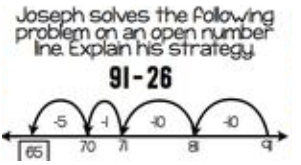
\includegraphics[width=1\linewidth]{images/numberline-add-sub-1a.png}
\end{image}%
 %
\item\hypertarget{li-502359792416}{} \begin{image}{0}{1}{0}%
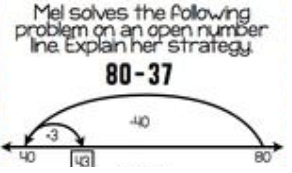
\includegraphics[width=1\linewidth]{images/numberline-add-sub-1b.png}
\end{image}%
 %
\end{enumerate}
\end{divisionexercise}%
\begin{divisionexercise}{2}{}{0.1}{exercise-502359790656}%
\hypertarget{p-502359789920}{}%
For each of the following, find the missing number by using an open number line (similar to those above).  Show at least two different methods for calculating the missing number on two different number lines.%
\leavevmode%
\begin{enumerate}[label=(\alph*)]
\item\hypertarget{li-502359788816}{}%
\begin{equation*}
42+?=91 
\end{equation*}
%
\item\hypertarget{li-502359788048}{}%
\begin{equation*}
57+?=83 
\end{equation*}
%
\end{enumerate}
\end{divisionexercise}%
\begin{divisionexercise}{3}{}{0.1}{exercise-502359786896}%
\hypertarget{p-502359786160}{}%
For the subtraction question%
\begin{equation*}
53-8\text{,}
\end{equation*}
Delia, a second grade student has done the following work:%
\begin{equation*}
53- 3=50-5=45
\end{equation*}
%
\leavevmode%
\begin{enumerate}[label=(\alph*)]
\item\hypertarget{li-502359784368}{}Explain how Delia came up with the numbers 3 and 5.%
\item\hypertarget{li-502359783888}{}Discuss Delia's method and answer to provide feedback.%
\item\hypertarget{li-502359783408}{}Use her method to answer the subtraction problem:%
\begin{equation*}
317-28
\end{equation*}
%
\end{enumerate}
\end{divisionexercise}%
\end{worksheet-section-numberless}
\restoregeometry
\end{chapterptx}
\end{document}